
\chapter{Knji"znica in gradniki za Orange}

V okviru diplomske naloge smo razvili tri lo"cene komponente za programerje in
kon"cne uporabnike programa Orange. 

Prva komponenta je programska knji"znica \verb|simple_wbd|, ki
omogo"ca enostaven dostop do programskega vmesnika indikatorjev in klimatskih
podatkov Svetovne banke. Ta knji"znica je narejena s "cim manj odvisnosti in je 
% TODO ali je python z veliko
namenjena splo"sni uporabi v Python programih. Poudarka pri zasnovi knji"znice 
\verb|simple_wbd| sta predvsem enostavnost razsiritve in zanesljivost. Ta cilja
dose"zemo z mehanizmom za vkljucevanje lastne kode v komponente knji"znice
in mehanizmi za popravljanje ali odstranjevanje pokvarjenih podatkov.

Drugi sestavni del je raz"siritev knji"znice \verb|simple_wbd| s 
funkcionalnostmi, potrebnimi za la"zje delo v programu Orange. To predvsem 
zavzema pretvorbo pridobljenih podatkov v podatkovno tabelo Orange in tabelo 
numpy. Ta sklop je namenjen skriptnemu delu s programom Orange 
\cite{orange_scripting} in je dostopen
kot \verb|api_wrapper| Python modul. 

Tretji sestavni del je grafi"cni vmesnik za uporabo \verb|api_wrapper| modula.
Namen grafi"cnega vmesnika je omogo"citi ne-programerjem dostop do podatkov 
programskega vmesnika Svetovne banke znotraj programa Orange za namen obdelave,
analize in iskanja zakonitosti v podatkih.

\section{Knji"znica simple\_wbd}

Knji"znica \verb|simple_wbd| programerjem olaj"sa dostop do podatkov 
programskega vmesnika Svetovne banke. Glavna lastnost te knji"znice je 
zdru"zevanje ve"cjega "stevila zahtev po podatkih in enostavna predstavitev 
prejetih podatkov. Druga lastnost je pretvorba podatkov iz ve"c dimenzij v 
dvo-dimenzionalno polje, primerno za uporabo v programu Orange. Glavna 
razreda te knji"znice sta \verb|IndicatorAPI| in \verb|ClimateAPI|. Prvi 
omogo"ca pridobivanje podatkov iz programskega vmesnika indikatorjev, drugi pa 
s programskega vmesnika podnebnih meritev.


"Ceprav za dostop do programskega vmesnika Svetovne banke "ze obstajajo 
re"sitve kot sta knji"znici 
\verb|wbdata|\fnurl{https://pypi.python.org/pypi/wbdata} in
\verb|wbpy|\fnurl{https://pypi.python.org/pypi/wbpy/2.0.1}, smo se odlo"cili
za lastno implementacijo podobne knji"znice. Glavni razlog za to je, da
obstoje"ce re"sitve posku"sajo "cim bolj natan"cno predstaviti programski
vmesnik Svetovne banke, ne pa olaj"sati dostop do "cim ve"cje koli"cine
podatkov.

Za potrebe te knji"znice smo razvili lastno re"sitev za predpomnenje poizvedb,
saj so se bolj splo"sne re"sitve, kot naprimer
\verb|vcrpy|\fnurl{https://pypi.python.org/pypi/vcrpy/1.10.0} in
\verb|requests-cache|\fnurl{https://pypi.python.org/pypi/requests-cache}, 
izkazale za prepo"casne ko delamo z ve"cjimi koli"cinami podatkov. Na"sa
re"sitev za predpomnenje izkori"sca dejstvo da je vsaka poizvedba dolo"cena le
z naslovom URL, in da so vsi odgovori oblike JSON. Za vsak URL naredimo novo
datoteko v sistemskem za"casnem imeniku, v kateri hranimo serializirane JSON
podatke. Ker se podatki na programskem vmesniku Svetovne banke redko
posodabljajo, smo za "cas veljavosti za"casnih datotek izbrali en teden.

% NOTE: serailizacija je baje uredu beseda:
% http://eprints.fri.uni-lj.si/2711/1/63100205-VALENTIN_KRAGELJ-Pregled_in_analiza_tehnologij_za_serializacijo_objektov.pdf

% server query je ful omojen (retarded) mi mamo bolsiga v guiju 

%% % moznost razsiritve z dedovanjem dataset razreda.
%% % 
%% 
%% - omogo"ca pridobivanje vrednosti za filtre:
%%     - indicator api: drzave in agregati, indikatorji
%%     - climate api: drzave, tipi podatkov, meritveno obdobje 
%% 
%% - Zahteva za podatke vraca dataset objekt ki ponuja surove podatke, ali pa eno
%%   drugo obliko. 2D array ali pa dict.
%% 
%% - Dataset razred lahko tudi poljubno razsirimo.



\subsection{Razred IndicatorAPI}

\verb|IndicatorAPI| je razred namenjen pridobivanju podatkov indikatorjev
razvoja dr"zav. Ker ima programski vmesnik Svetovne banke omejitev koliko 
podatkov lahko prenesemo z eno poizvedbo in nam dovoli tvoriti poizvedbe le za
en indikator na enkrat, smo napisali razred, ki v ozadju tvori in izvede
poizvedbe za vse strani vseh zahtevanih indikatorjev. To poskrbi tako da se po
prvi poizvedbi za en indikator sprehodi "cez "stevilo preostalih strani 
(Primer \ref{basic_response}), ki so na voljo, in pridobljene podatke ve"cih
strani zdru"zi in predstavi kot rezultat ene same poizvedbe. Ta postopek ponovi
za vse zahtevane indikatorje, in njihove rezultate vrne v obliki slovarja, ki 
ima za klju"c kodo indikatorja posamezne zahteve.

Poleg tega da skrbi za prenos vseh strani podatkov, tudi bele"zi "stevilo 
izvedenih in "stevilo potrebnih poizvedb za celoten prenos. Ta "stevila se
lahko uporablja za prikaz napredka prenosa podatkov.


Za namene razreda \verb|IndicatorAPI| smo v knji"znici \verb|simple_wbd|
razvili mehanizvme za odpravo nekaterih napak omenjenih v poglavju 
\ref{api_gotchas}.

Pri manjkajo"cih vrednostih dr"zav v poizvedbah za podatke indikatorjev,
posku"samo dolo"citi pravilne vrednosti. To naredimo s pomo"cjo dveh
slovarjev: prvi slika kode dr"zav v imena, drugi pa imena dr"zav v kode. V
primeru manjkajo"ce vrednosti kode ali imena, posku"samo to prebrati iz enega
od na"stetih slovarjev. "Ce nam ne uspe ugotoviti manjkajo"cih vrednosti,
trenutni vnos odstranimo iz rezultata poizvedbe.

Drugi tip napak, ki ga lahko delno popravimo, so napa"cne vrednosti v polju
\verb|date| v poizvedbah za podatke indikatorjev. Ker lahko v temu polju
pri"cakujemo poljubeno besedilo, dela na"s pretvornik za polje \verb|date| v 
datum, tako da posku"sa v datum pretvoriti "cim dalj"so predpono besedila.
"Ce nam ne uspe besedila pretvoriti v veljaven datum, trenutni vnos odstranimo
iz rezultata poizvedbe.


\ \\
Glavne metode ki jih ponuja razred IndicatorAPI so:

\begin{description}  
\item [get\_indicators] za pridobivanje seznama indikatorjev s kodami, imeni
      in opisi,
\item [get\_countries] za pridobivanje seznama drzav z metapodatki,
\item [get\_dataset] za pridobivanje podatkov za indikatorjev.
\end{description}


\subsubsection{Razred IndicatorDataset}

Razred \verb|IndikatorDataset| je osnovni razred v katerem dobimo zahtevane podatke
indikatorjev. Ta razred vsebuje vse potrebne metode in podatke za predstavitev
rezultatov programskega vmesnika, na dva glavna na"cina; kot slovar slovarjev in
dvo dimenzionalen seznam. Poleg omenjenih na"cinov predstavitve podatkov lahko
dostopamo tudi do neobdelanih podatkov prejetih z programskega vmesnika za
vsako poizvedbo posebej.


Posamezne vrednosti teh podatkov so dolo"cene z drzavo, casovno komponento, in
kodo indikatorja. Te podatke lahko predstavimo na dva glavna nacina:

 - kot gnezdeni slovar, kjer je na prvem nivoju ime indikatorja, na drugem
   drzava, in na tretjem nivoju casovna komponenta.

 - Kot dvo-dimenzionalno polje, kjer imamo v vrsticah eno oznako, v stolpcih
   pa kartezicni produkt ostalih dveh. ponujene moznosti so:
   - vrstice = drzava, stolpci = cas x indikator
   - vrstice = cas, stolpci = drzava x indikator


Indicator



% notes:
% 3 dimenzije: cas, drzava, indikator > vrednost
% 
% lahko damo v:
% 
% 
%    \    drzava x indikator
%   cas
% 
%  ali: 
% 
%    \    cas x indikator
% drzava
% 


\subsubsection{Primeri uporabe}





\subsection{Pomcnik ClimateAPI}

IndicatorAPI je 


api dovoli le podatke za en tip za eno vrsto obdobja in eno drzavo hkrati.
mi naredim kartezicni produkt med vsemi temi zgradimo vse url-je in naredimo
vse potrebne poizvedbe za pridobitev podatkov.



\subsubsection{Razred IndicatorDataset}

Isto kot pri indicator apiju
ko zelimo dobiti polje v obliki casovne vrste:
 - pridobivanje datuma iz polja 'date'
   - ob neveljavnih stringih probamo upostevati le zacetni del.
     - za text za  obdobje  '2002 - 2006' bomo uporabili le datum 2002 
   - neveljavne stringe kot so "most rescent value" ignoriramo.




as\_dict 

glede na poizvedbo dobimo tu gnezden slovar s polji

drzava / tip podatkov / tip casovnega obdobja / vrednost casovnega obdobja / vrednost

as\_list

% notes:
% 3 dimenzije: cas (decade,year,month), drzava, tip (pr/ tas)
% 
% lahko damo v poljubno konfiguracijo z nastetimi elementi v stolpcu
% 
% stolpci = [drzava, cas] => vrstice = tip ... naredi kartezicni produkt



\section{api\_wrapper}

% doda as orange table in as numpy obema indikator apiju in climate apiju.


raz"siritev simple wbd vmesnikov z dedovanjem pravega dataset razreda.

\begin{verbatim}

class ClimateDataset(simple_wbd.ClimateDataset):
    
    def as_numpy(self):
        raise NotImplemented()
    
    def as_orange_table(self):
        raise NotImplemented()

class ClimateAPI(simple_wbd.ClimateAPI):

    def __init__(self):
        super().__init__(ClimateDataset)
\end{verbatim}


- razsiri as\_list v as\_numpy\_array ki tudi odstrani vse stolpce ki nimajo 
  veljavne vrednosti.

- doda as orange table ki numpy array spremeni v orange tabelo.
  - za indikator api doda se metapodatke drzav ko ne prikazujemo v obliki casovne vrste.


api vrapper je tudi zelo uporaben za skriptno uporaba programa Orange 
(referenca http://www.jmlr.org/papers/volume14/demsar13a/demsar13a.pdf)

in tukaj si lahko vsak programer sam oblikuje podatke v katerokoli zeljeno obliko.






\section{Graficni vmesnik}


 
nova skupina data sets 
 - v katero je mogoce dodati nove gradnike za druge programske vmesnike.

2 gradnika - wb indicators in wb climate

- lazja uporaba apija
- vecja preglednost


za oba gradniko smo razvili in uporabili base class - skupni podatki

- razvili smo tudi gradnik za gnezned prikaz urejenih slovarjev.
  ta se uporablja za prikaz drzav po kontinentih v climate gradniku,
  in za prikaz drzav in skupin drzav in drugih agregatov v gradniku
  indicators.


za te gradnike smo tudi napisali enotske teste.


\begin{figure}
  \begin{center}
    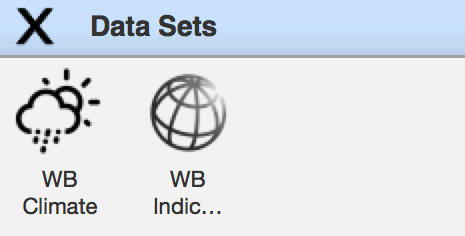
\includegraphics[width=4cm]{pic/data_sets_group.png}
  \end{center}
  \caption{Skupina gradnikov data sets}
  \label{drevo}
\end{figure} 


\subsection{wb indicators gradnik}

za sestavo smo si pomagali z gradniki Orange.gui 

elementi gradnika

2 osnovna filtra: 

- izbor indikatorjev ki se pokazejo v seznamu all/common/featured 
  ki ustreza seznamu indikatorjev na strani: 
  all - vse (tudi nekateri ki jih na strani ni nastetih)
  common - http://data.worldbank.org/indicator?tab=all
  featured - http://data.worldbank.org/indicator?tab=featured
- text filter

gradnik ima sistem za prikaz (progress bar?) 

moznost izbire tipa izhoda (countries in time series - opis)

\begin{figure}
\begin{center}
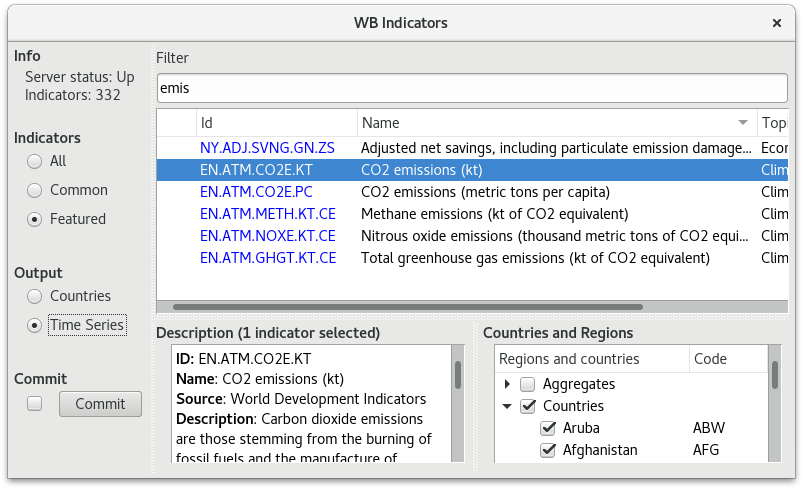
\includegraphics[width=12cm]{pic/co2_temp_indicator_selection.png}
\end{center}
\caption{Odločitveno drevo za izbor primerne metode.}
\label{co2_temp_indicator}
\end{figure} 



\subsection{wb climate gradnik}

dovoli izbiro posameznih drzav 

moznost izbire tipa izhoda (countries in time series - opis)
za razliko od indikator apija tukaj nismo dodali metapodatkov drzav 



\begin{figure}
\begin{center}
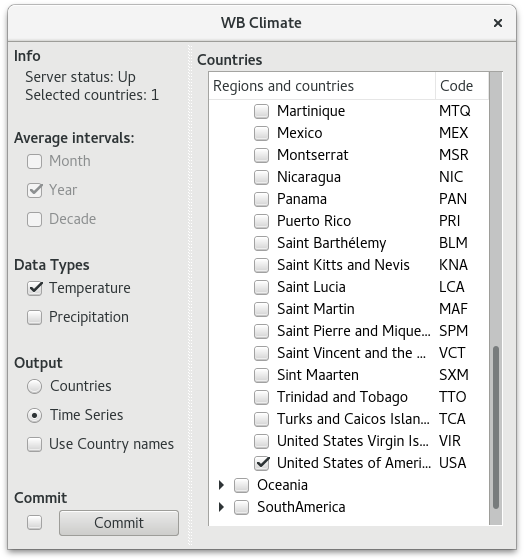
\includegraphics[width=12cm]{pic/co2_temp_climate_selection.png}
\end{center}
\caption{Odločitveno drevo za izbor primerne metode.}
\label{co2_temp_indicator}
\end{figure} 
